%-------------------------------------------------------------------------------
%-------------------------------------------------------------------------------
\begin{frame}\begin{center}
	\LARGE\textbf{Objects of interest}
\end{center}\end{frame}
%-------------------------------------------------------------------------------
%-------------------------------------------------------------------------------
\begin{frame}
	\textbf{Useful Notation}
	\begin{align*}
		P(X, Z) & = \Pr(D = 1\mid X, Z) = F_V(\mu_D(X, Z)) \\
		U_D     & = F_V(V)
	\end{align*}

\end{frame}

%-------------------------------------------------------------------------------
%-------------------------------------------------------------------------------
\begin{frame}
\begin{figure}[htp]\centering\caption{First-stage unobservable}
\scalebox{0.35}{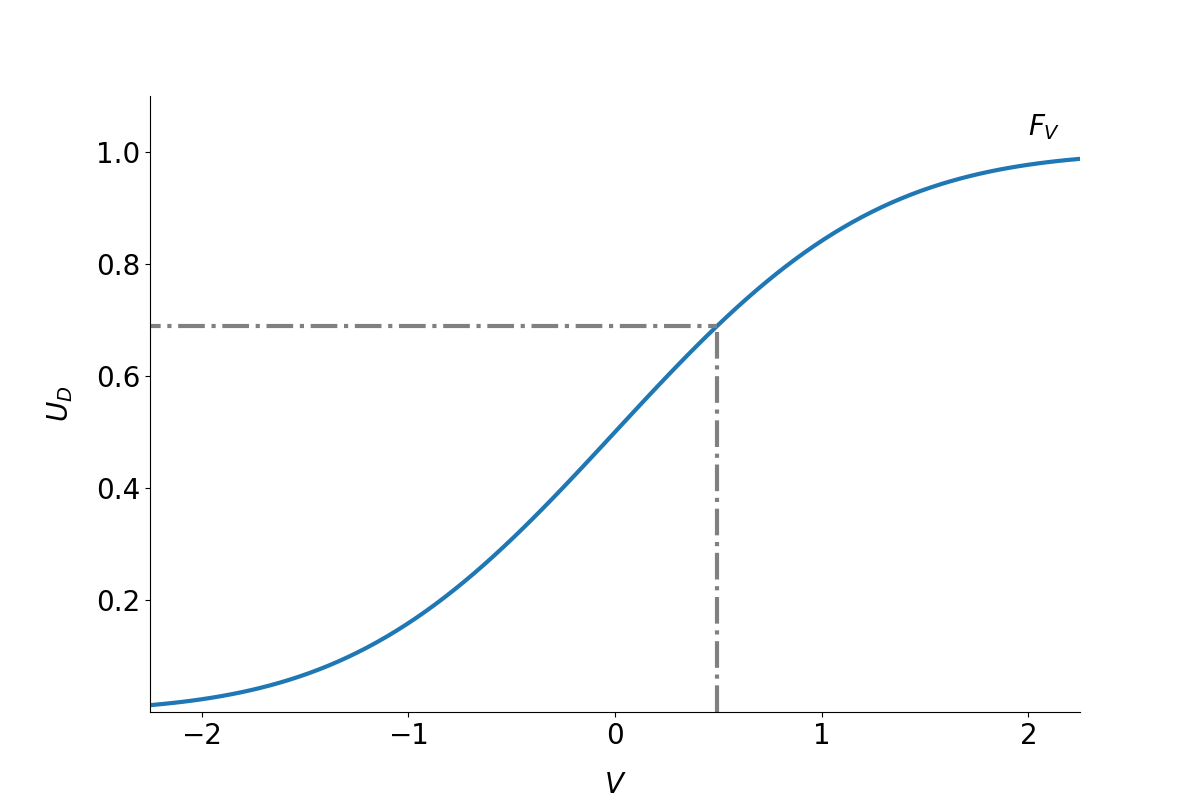
\includegraphics{fig-quantile-function.png}}
\end{figure}
\end{frame}
%-------------------------------------------------------------------------------
%-------------------------------------------------------------------------------
\begin{frame}
\begin{figure}[htp]\centering\caption{Support}
\scalebox{0.35}{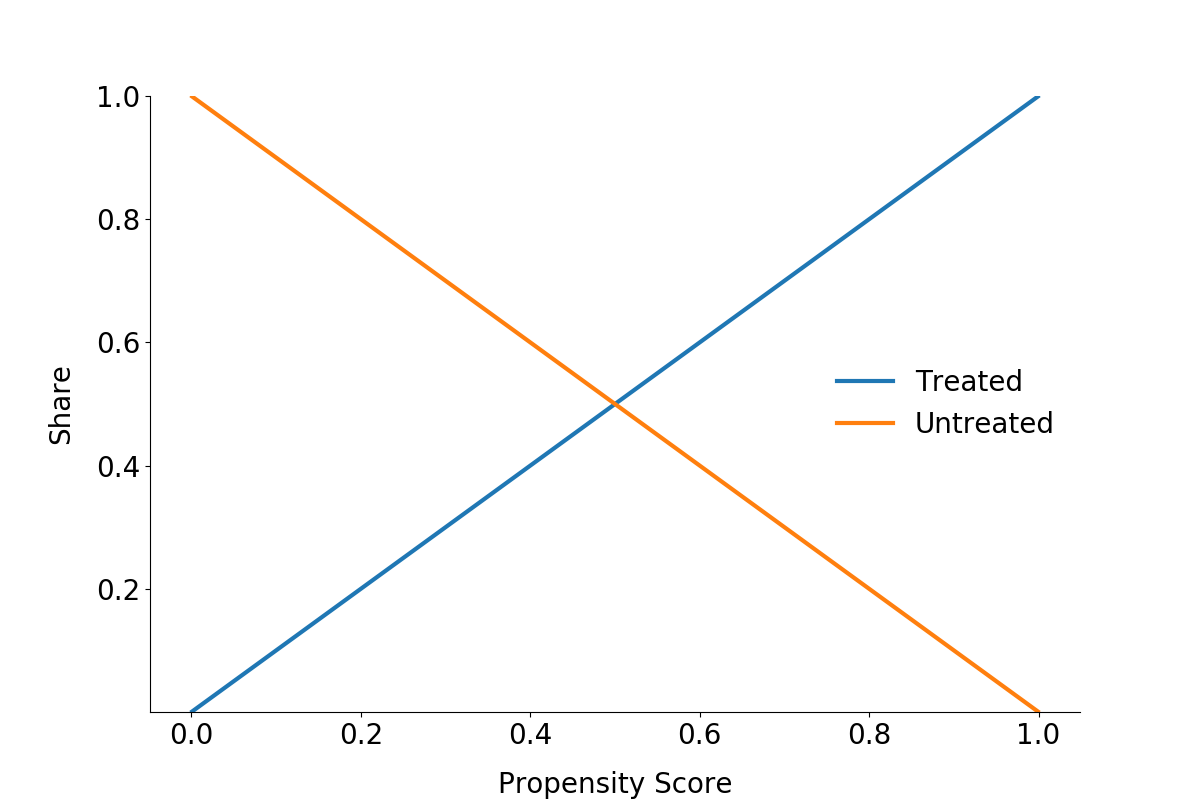
\includegraphics{fig-common-support-stylized.png}}
\end{figure}
\end{frame}

%-------------------------------------------------------------------------------
%-------------------------------------------------------------------------------
\begin{frame}
\begin{figure}[htp]\centering\caption{Distribution of benefits}
\scalebox{0.35}{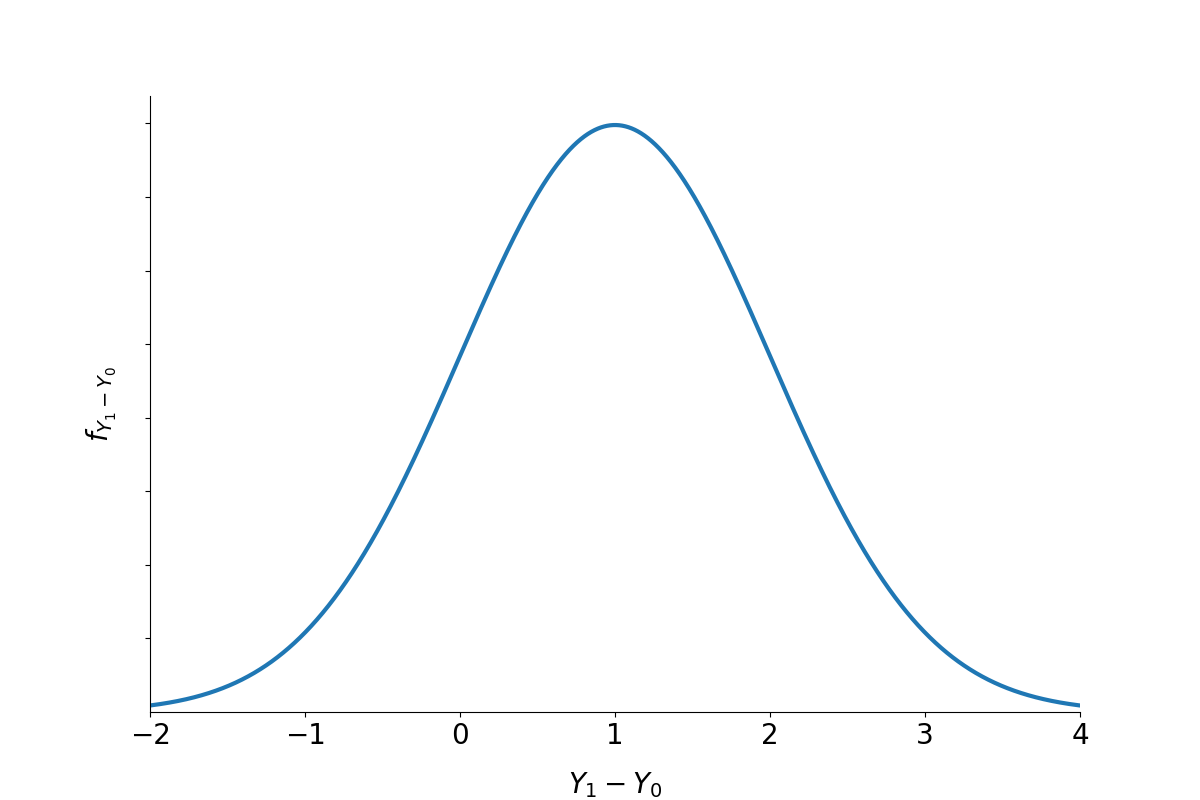
\includegraphics{fig-treatment-effects-benefits}}
\end{figure}
\end{frame}
%-------------------------------------------------------------------------------
%-------------------------------------------------------------------------------
\begin{frame}
	\begin{figure}\caption{Conditional expectation and essential heterogeneity}
		\scalebox{0.35}{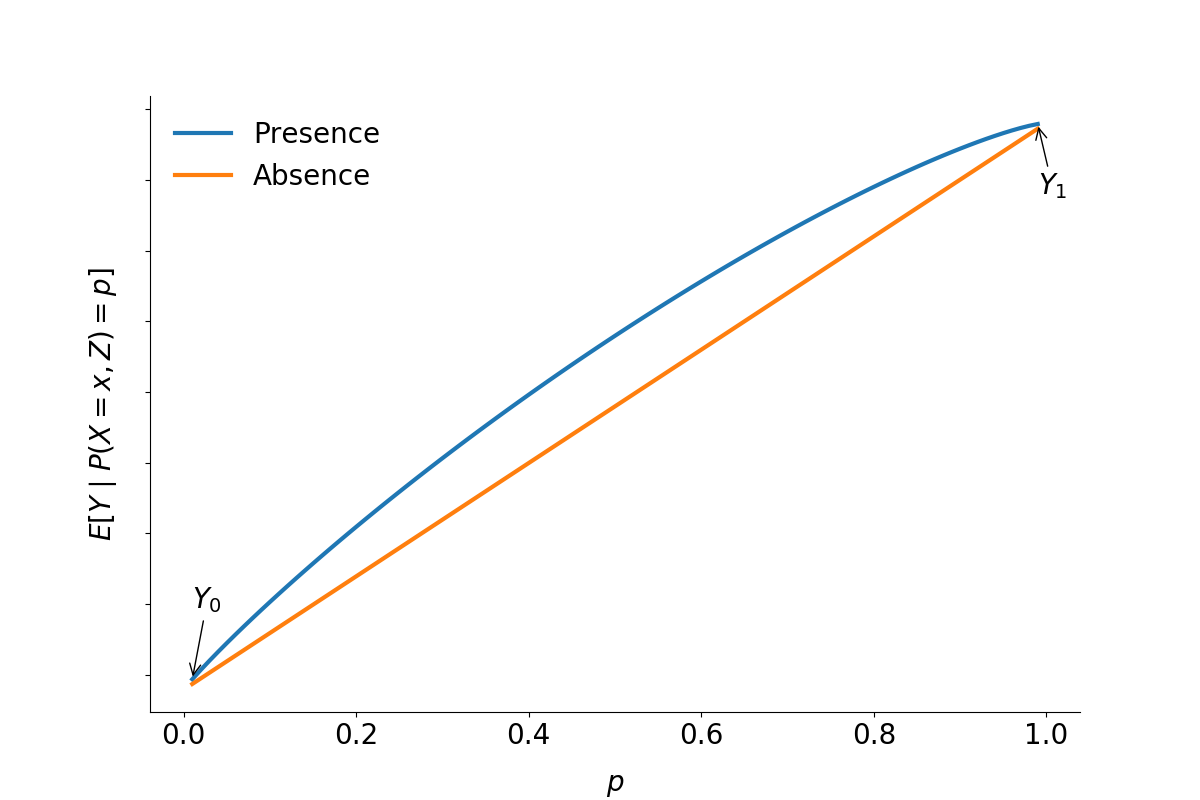
\includegraphics{fig-eh-conditional-expectation}}
	\end{figure}
\end{frame}
%-------------------------------------------------------------------------------
%-------------------------------------------------------------------------------
\begin{frame}\begin{center}
		\LARGE\textit{Conventional Average Treatment Effects}
\end{center}\end{frame}
%-------------------------------------------------------------------------------
%-------------------------------------------------------------------------------
\begin{frame}
	\textbf{Conventional Average Treatment Effects}
	\begin{align*}
		B^{ATE} & = E[Y_1 - Y_0 ]\\
		B^{TT} & = E[Y_1 - Y_0 \mid D = 1]\\
		B^{TUT} & = E[Y_1 - Y_0 \mid D = 0]\\
	\end{align*}
	\(\Rightarrow\) correspond to \emph{extreme} policy alternatives
\end{frame}
%-------------------------------------------------------------------------------
%-------------------------------------------------------------------------------
\begin{frame}
\textbf{Selection Problem}

	\begin{align*}
		E[Y\mid D = 1] - E[Y\mid D = 0] & = \underbrace{E[Y_1 - Y_0\mid D = 1]}_{B^{TT}} \\
		& + \underbrace{E[Y_0\mid D= 1]- E[Y_0 \mid D = 0]}_{\text{Selection bias}}
	\end{align*}
\end{frame}
%-------------------------------------------------------------------------------
%-------------------------------------------------------------------------------
\begin{frame}
	\begin{align*}
		E[Y\mid D = 1] - E[Y\mid D = 0] & = \underbrace{E[Y_1 - Y_0]}_{B^{ATE}} \\
		& + \underbrace{E[Y_1 - Y_0 \mid D = 1] - E[Y_1 - Y_0]}_{\text{Sorting on gains}} \\
		& + \underbrace{E[Y_0\mid D = 1] - E[Y_0 \mid D = 0]}_{\text{Sorting on levels}}
	\end{align*}
\end{frame}
%-------------------------------------------------------------------------------
%-------------------------------------------------------------------------------
\begin{frame}
	\begin{itemize}\setlength\itemsep{1em}
	\item bias depends on the parameter of interest
	\item selection bias as sorting on levels
	\end{itemize}
\end{frame}

%-------------------------------------------------------------------------------
%-------------------------------------------------------------------------------
\begin{frame}
	\begin{figure}\caption{Distribution of effects with essential heterogeneity}
		\scalebox{0.35}{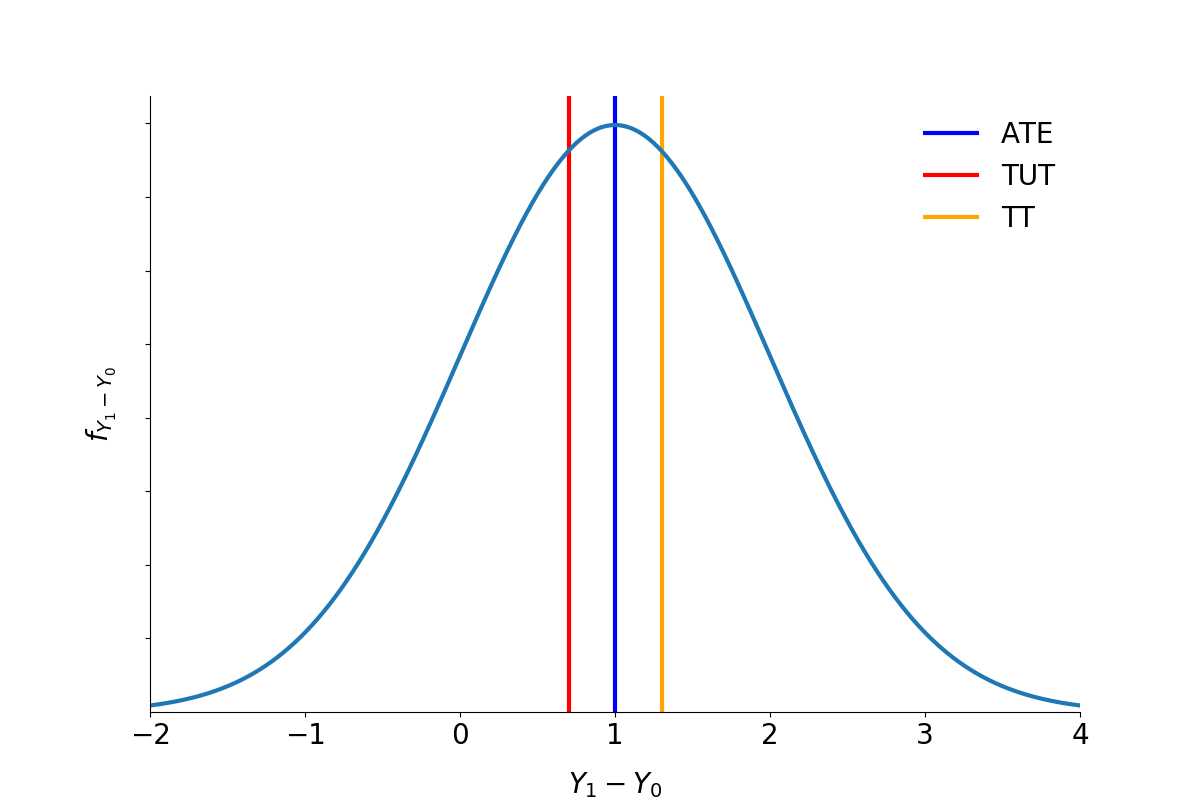
\includegraphics{fig-treatment-effects-with-eh}}
	\end{figure}
\end{frame}
%-------------------------------------------------------------------------------
%-------------------------------------------------------------------------------
\begin{frame}
	\begin{figure}\caption{Distribution of effects without essential heterogeneity}
		\scalebox{0.35}{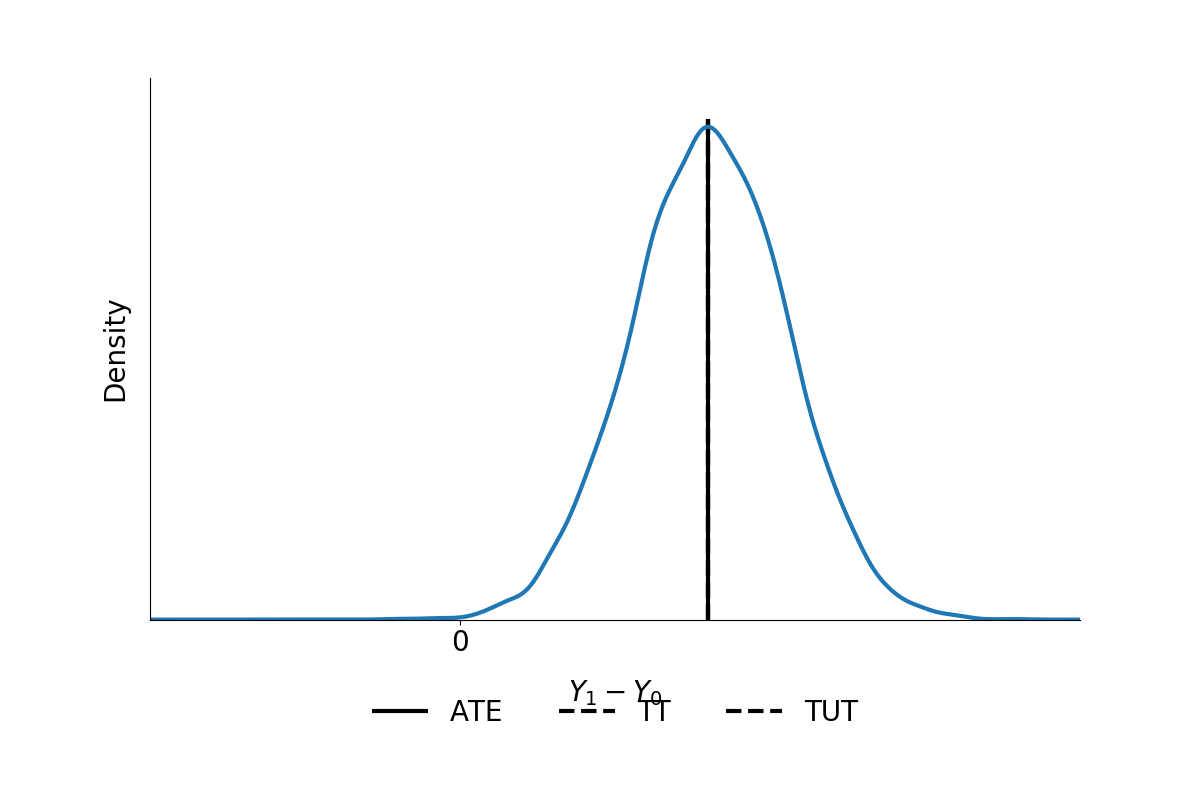
\includegraphics{fig-treatment-effects-without-eh}}
	\end{figure}
\end{frame}
%-------------------------------------------------------------------------------
%-------------------------------------------------------------------------------
\begin{frame}\begin{center}
		\LARGE\textit{Policy-Relevant Average Treatment Effects}
\end{center}\end{frame}
%-------------------------------------------------------------------------------
%-------------------------------------------------------------------------------
\begin{frame}
	\textbf{Observed Outcomes}
	\begin{align*}
		Y_B = D_B Y_1 + (1 - D_B) Y_0 \\
		Y_A = D_A Y_1 + (1 - D_A) Y_0 \\
	\end{align*}
	\textbf{Effect of Policy}
	\begin{align*}
		B^{PRTE} = \frac{1}{E[D_A] - E[D_B]} (E[Y_A] - E[Y_B])
	\end{align*}
\end{frame}
%-------------------------------------------------------------------------------
%-------------------------------------------------------------------------------
\begin{frame}\begin{center}
		\LARGE\textit{Marginal Benefit of Treatment}
\end{center}\end{frame}
%-------------------------------------------------------------------------------
%-------------------------------------------------------------------------------
\begin{frame}\textbf{Marginal Benefit of Treatment}
	\begin{align*}
		B^{MTE}(x, u_D) = E [Y_1 - Y_0 \mid X = x,  U_D = u_D]
	\end{align*}
	\textbf{Intuition:} Mean gross return to treatment for persons at
	quantile \(u_D\) of the first-stage unobservable \(V\) or a willingness to pay for individuals at the margin of indifference.
\end{frame}
%-------------------------------------------------------------------------------
%-------------------------------------------------------------------------------
\begin{frame}
	\begin{figure}\caption{Margin of indifference}
		\scalebox{0.35}{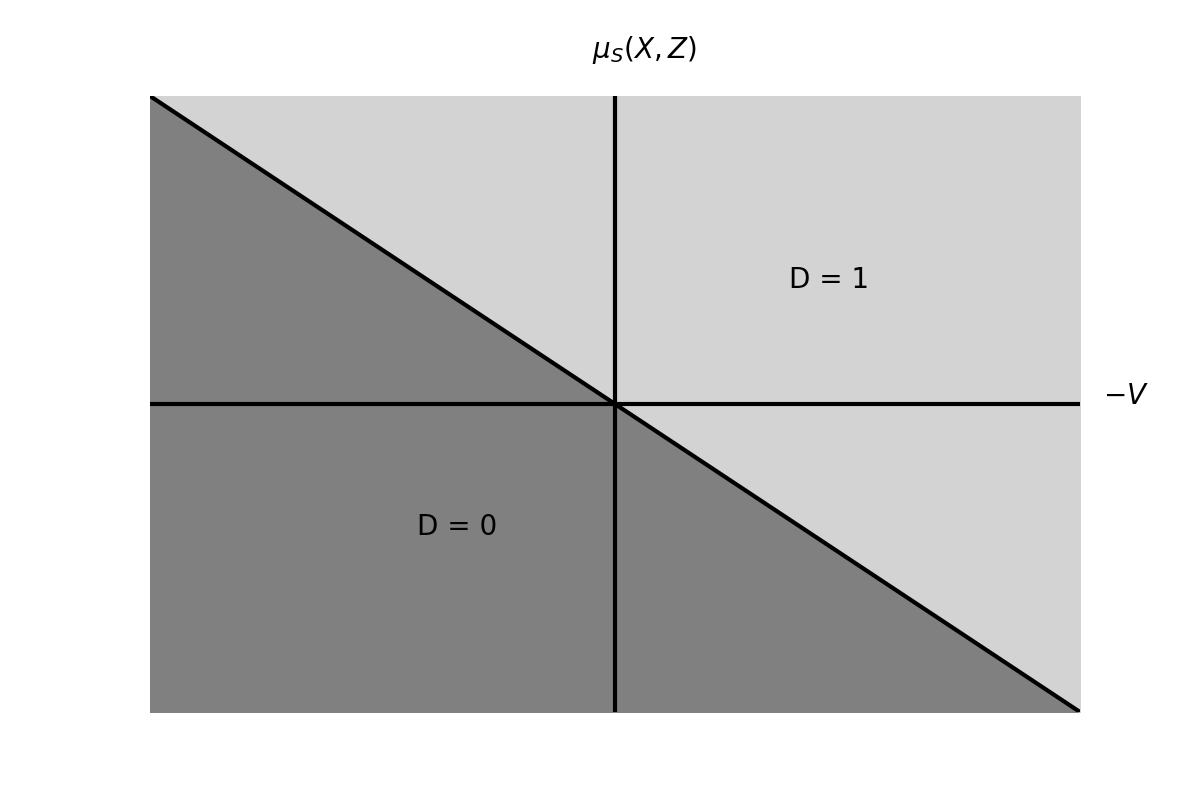
\includegraphics{fig-margin-indifference}}
	\end{figure}
\end{frame}
%-------------------------------------------------------------------------------
%-------------------------------------------------------------------------------
\begin{frame}
\begin{figure}\caption{$B^{MTE}$ and essential heterogeneity}
		\scalebox{0.35}{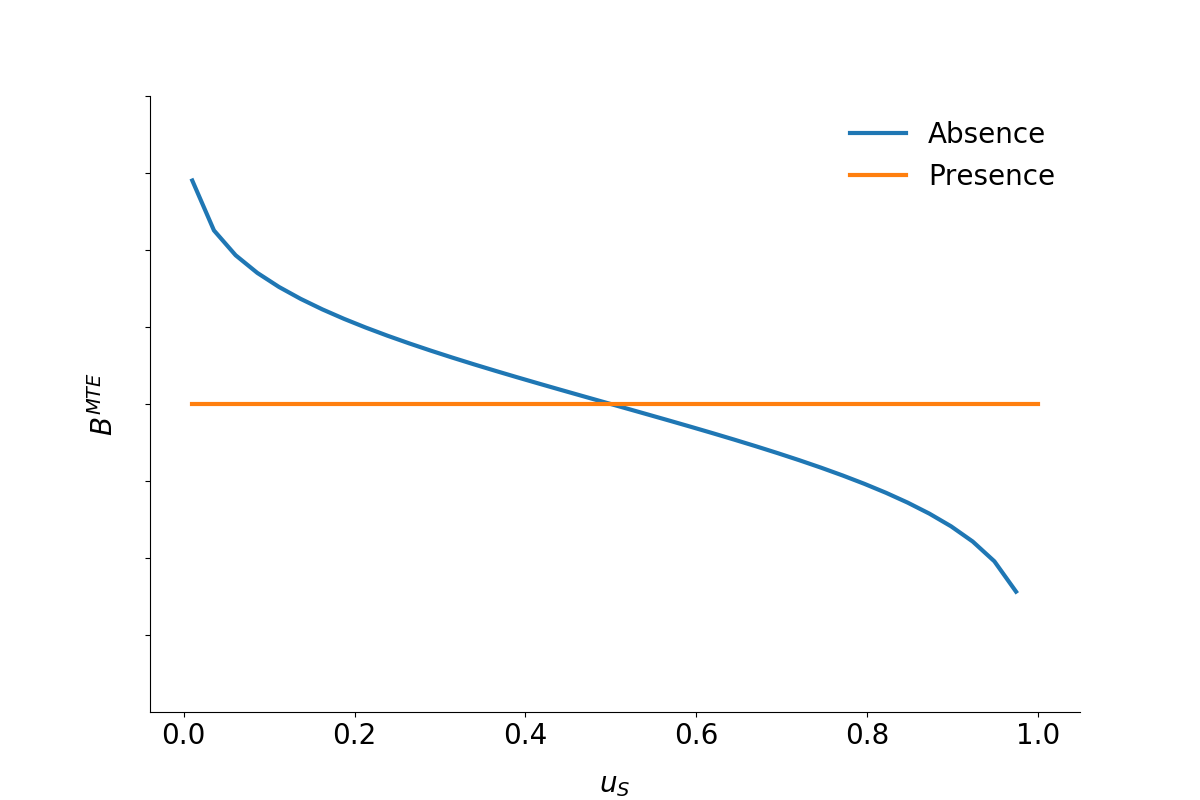
\includegraphics{fig-eh-marginal-effect}}
	\end{figure}
\end{frame}
%-------------------------------------------------------------------------------
%-------------------------------------------------------------------------------
\begin{frame}
	\begin{figure}\caption{Selection scenarios}
		\scalebox{0.35}{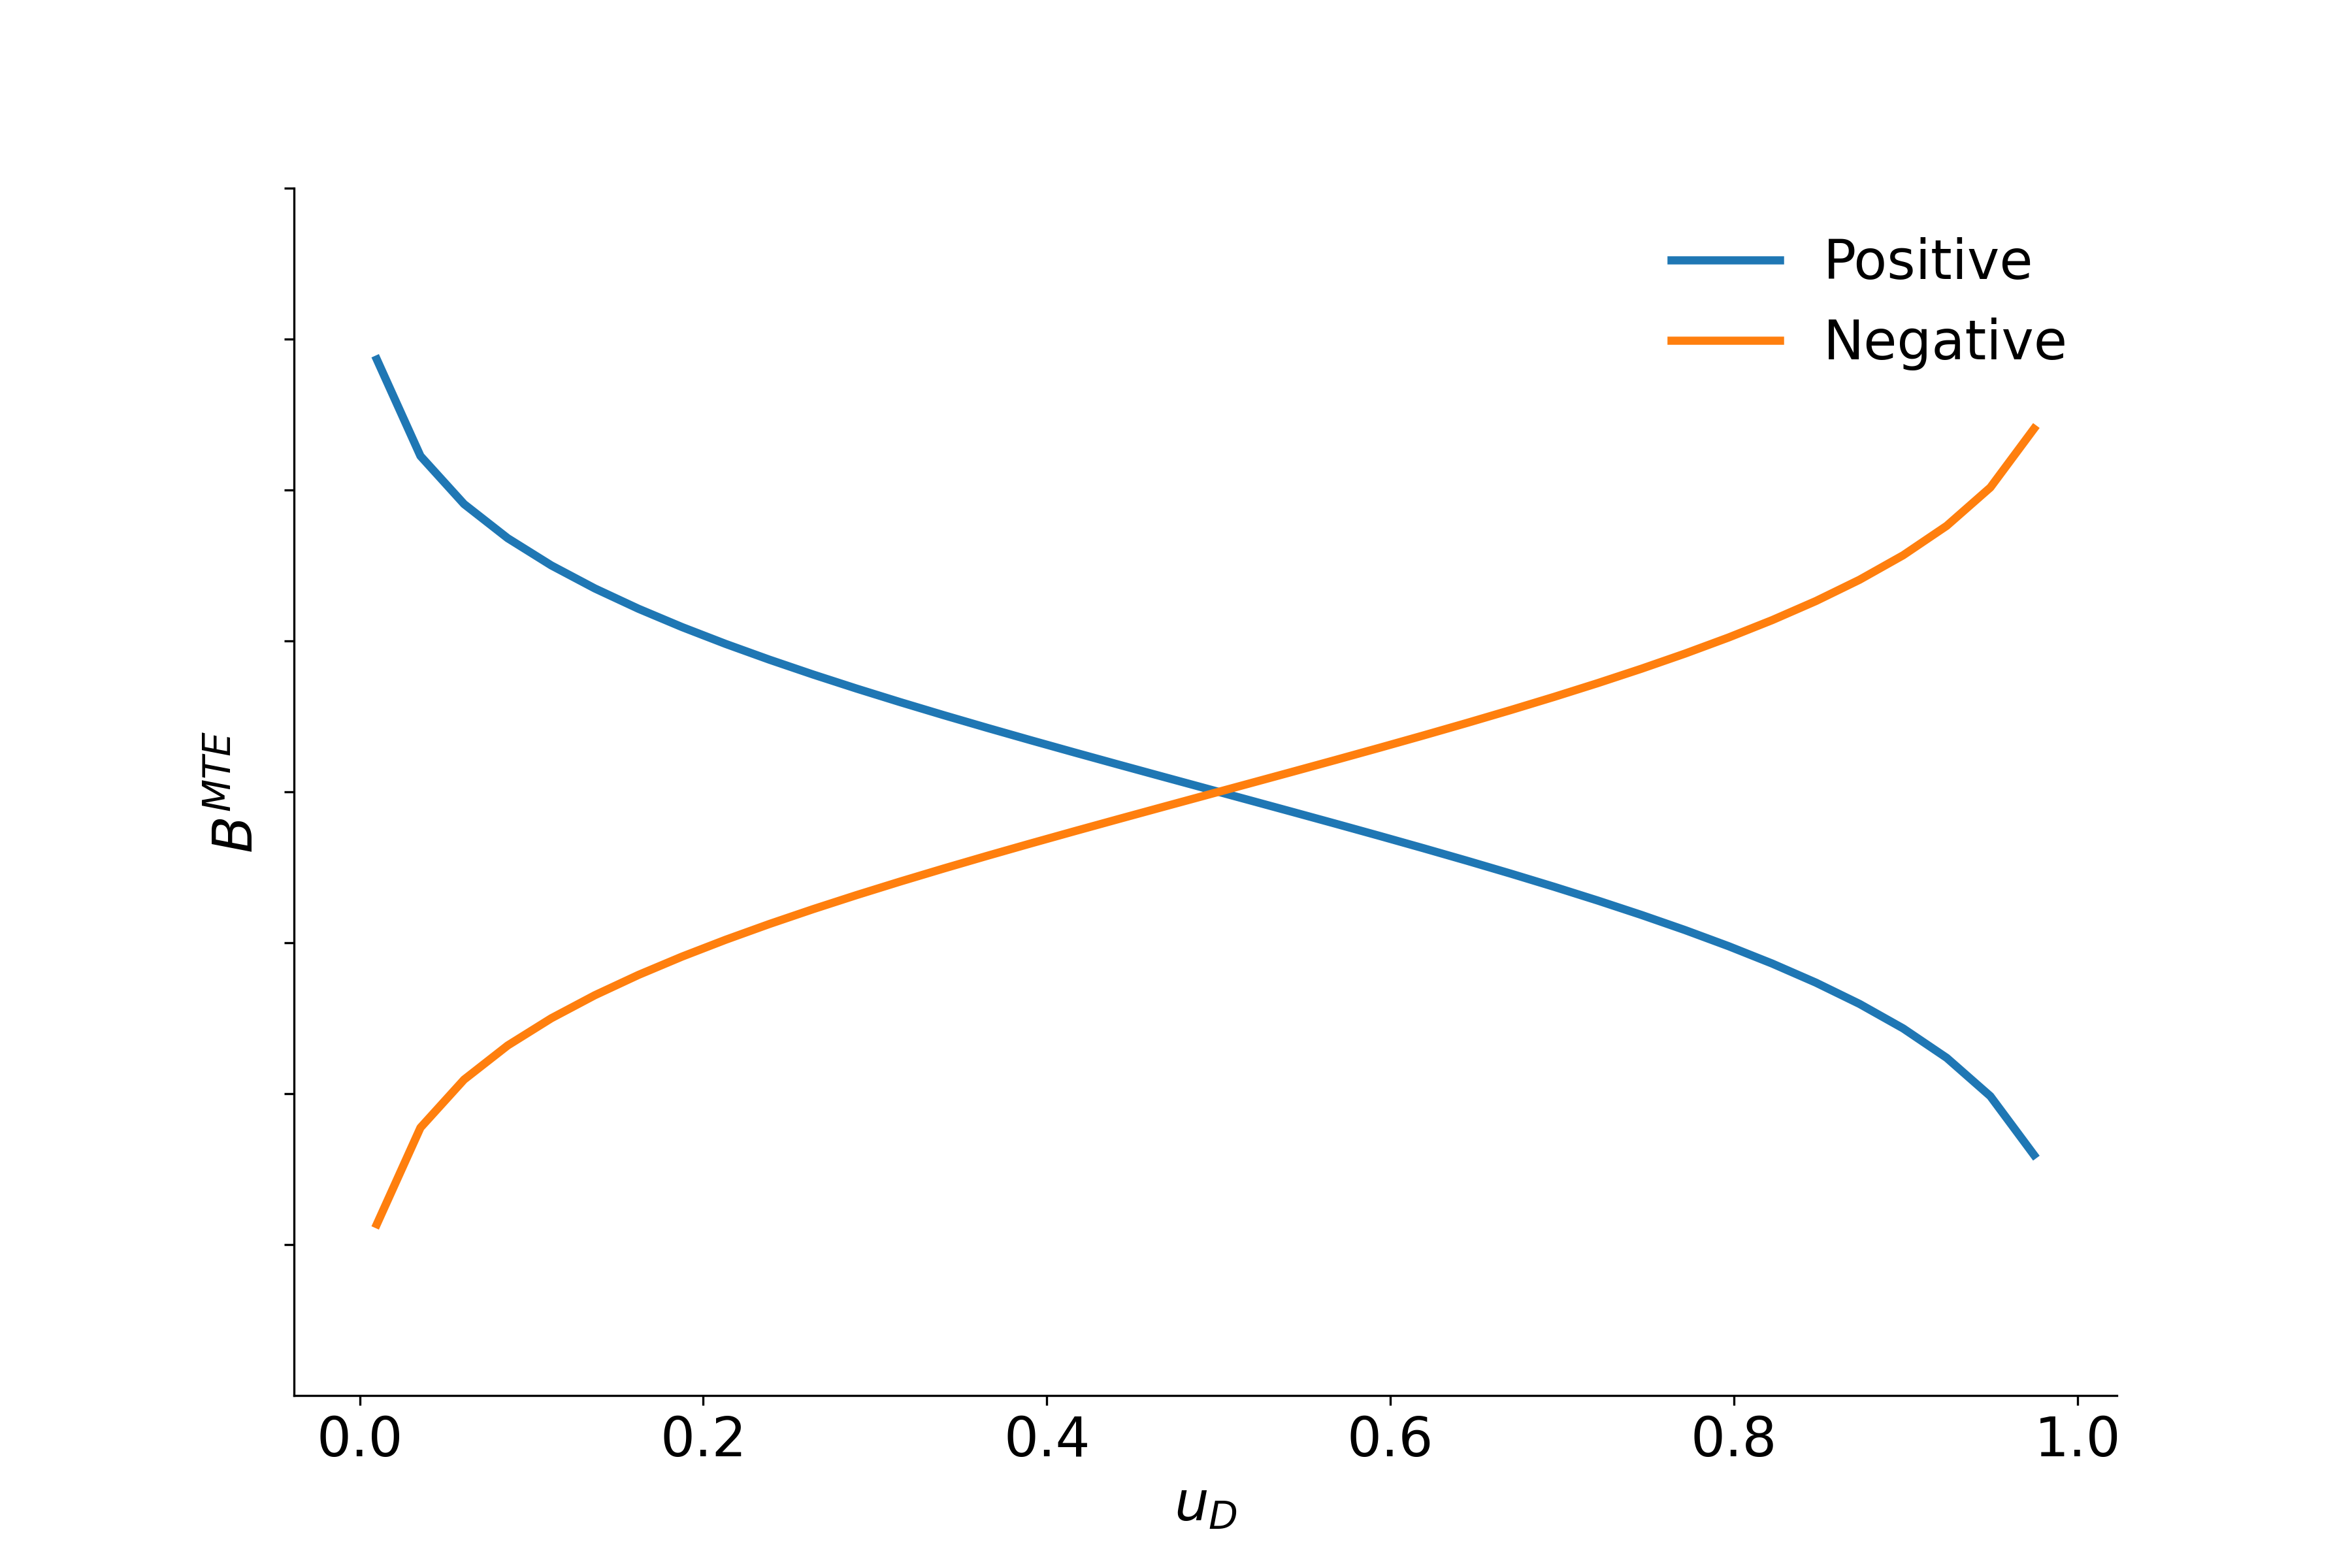
\includegraphics{fig-marginal-effect-scenarios}}
	\end{figure}
\end{frame}
%-------------------------------------------------------------------------------
%-------------------------------------------------------------------------------
\begin{frame}
	\textbf{Effects of treatment as weighted averages}
	Parameter \(\Delta_j\), can be written as a weighted average of the
	\(B^{MTE}(x, u_D)\).
	\begin{align*}
		\Delta_j(x) = \int_0^1 B^{MTE}(x, u_D) \omega^j(x, u_D) du_D,
	\end{align*}
	where the weights \(\omega^j(x, u_D)\) are specific to parameter \(j\)
	and integrate to one.
\end{frame}
%-------------------------------------------------------------------------------
%-------------------------------------------------------------------------------
\begin{frame}
	\textbf{Weights}
	\begin{align*}
		\omega^{ATE}(x, u_D) & = 1 \\
		\omega^{TT}(x, u_D) & = \frac{1 - F_{P\mid X=x}(u_D)}{E[P \mid X = x]}\\
		\omega^{TUT}(x, u_D) & = \frac{F_{P\mid X=x}(u_D)}{E[1 - P \mid X = x]}
	\end{align*}
\end{frame}
%-------------------------------------------------------------------------------
%-------------------------------------------------------------------------------
\begin{frame}
	\begin{figure}\caption{Effects of treatment as weighted averages}
		\scalebox{0.35}{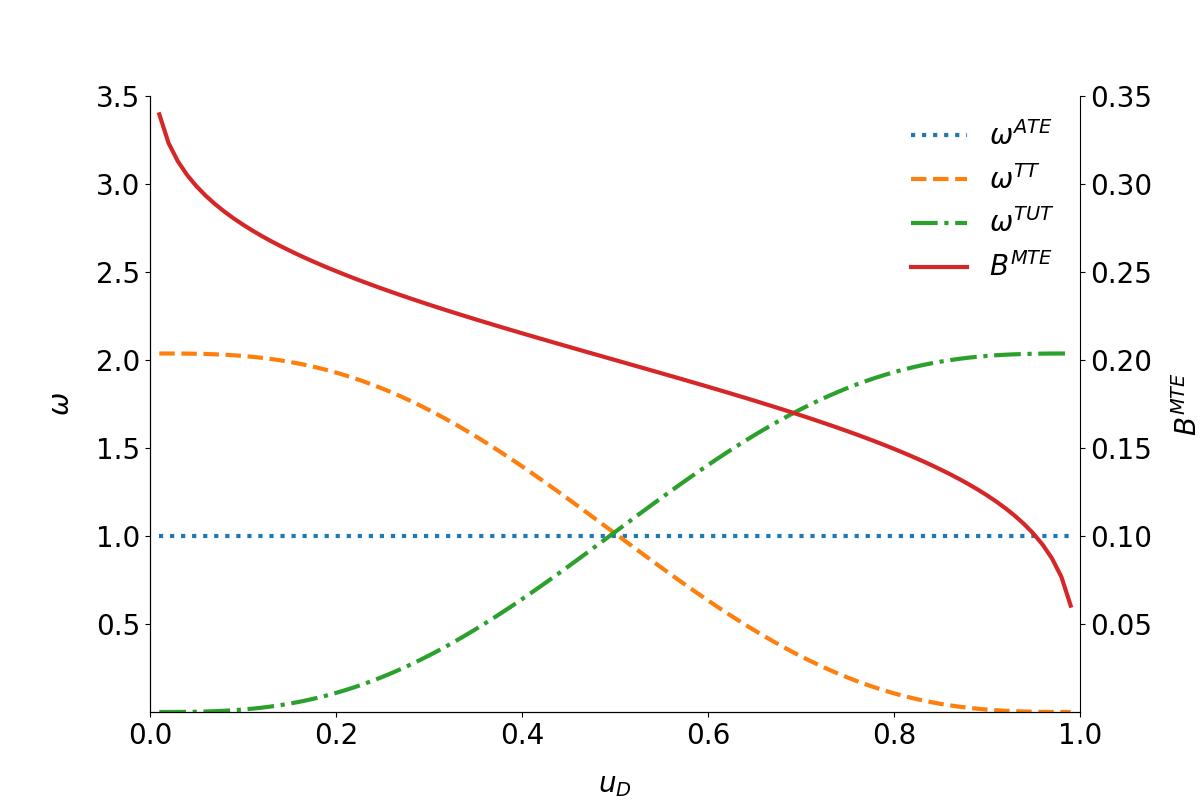
\includegraphics{fig-weights-marginal-effect}}
	\end{figure}
\end{frame}
%-------------------------------------------------------------------------------
%-------------------------------------------------------------------------------
\begin{frame}\begin{center}
		\LARGE\textit{Local Average Treatment Effect}
\end{center}\end{frame}
%-------------------------------------------------------------------------------
%-------------------------------------------------------------------------------
\begin{frame}\textbf{Local Average Treatment Effect}\vspace{0.3cm}
	\begin{itemize}\setlength\itemsep{1em}
		\item \textbf{Local Average Treatment Effect:} Average effect for those induced
		to change treatment because of a change in the instrument.\\\vspace{0.2cm}
		\(\Rightarrow\) instrument-dependent parameter\vspace{0.4cm}

		\item \textbf{Marginal Treatment Effect:} Average effect for those individuals
		with a given unobserved desire to receive treatment.\\\vspace{0.2cm}
		\(\Rightarrow\) deep economic parameter
	\end{itemize}
\end{frame}
%-------------------------------------------------------------------------------
%-------------------------------------------------------------------------------
\begin{frame}
	\begin{align*}
		B^{LATE} = \frac{E[Y\mid Z = z] - E[Y \mid Z = z^\prime]}{P(z) - P(z^\prime)}
	\end{align*}
	\begin{align*}
		B^{LATE}(x, u_D, u_{D^\prime}) = \frac{1}{u_D - u_{D^\prime}} \int_{u_D}^{u_{D^\prime}} B^{MTE}(x, u) du,
	\end{align*}
\end{frame}
%-------------------------------------------------------------------------------
%-------------------------------------------------------------------------------
\begin{frame}
	\begin{figure}[htp]\centering
		\caption{Local average treatment effect}\scalebox{0.35}
		{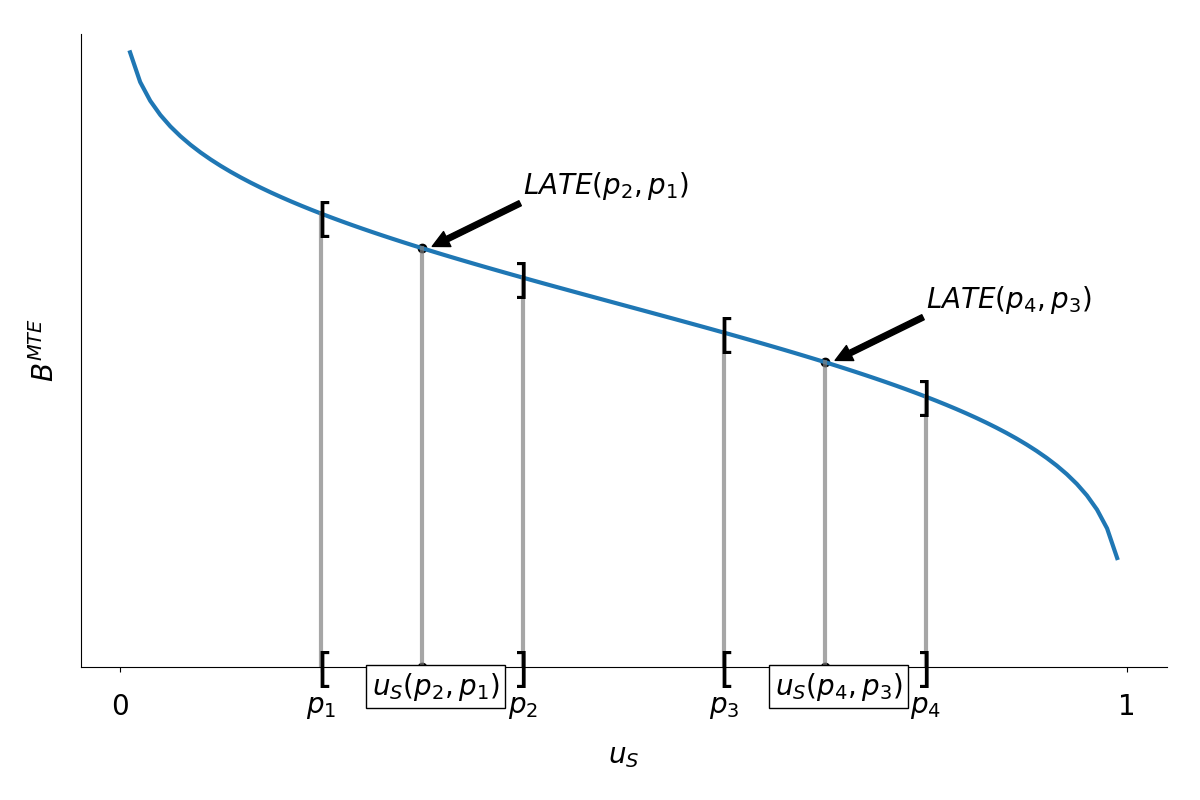
\includegraphics{fig-local-average-treatment}}
	\end{figure}
\end{frame}

%-------------------------------------------------------------------------------
%-------------------------------------------------------------------------------
\begin{frame}\begin{center}
		\LARGE\textit{Distributions of Effects}
\end{center}\end{frame}


%-------------------------------------------------------------------------------
%-------------------------------------------------------------------------------
\begin{frame}\textbf{Distrbutions of Effects}\vspace{0.3cm}
\begin{itemize}\setlength\itemsep{1em}
	\item marginal distribution of benefits
	\item joint distribution of potential outcomes
	\item joint distribution of benefits and surplus
\end{itemize}\end{frame}
%-------------------------------------------------------------------------------
%-------------------------------------------------------------------------------
\begin{frame}
\begin{figure}[htp]\centering\caption{Distribution of benefits}
\scalebox{0.35}{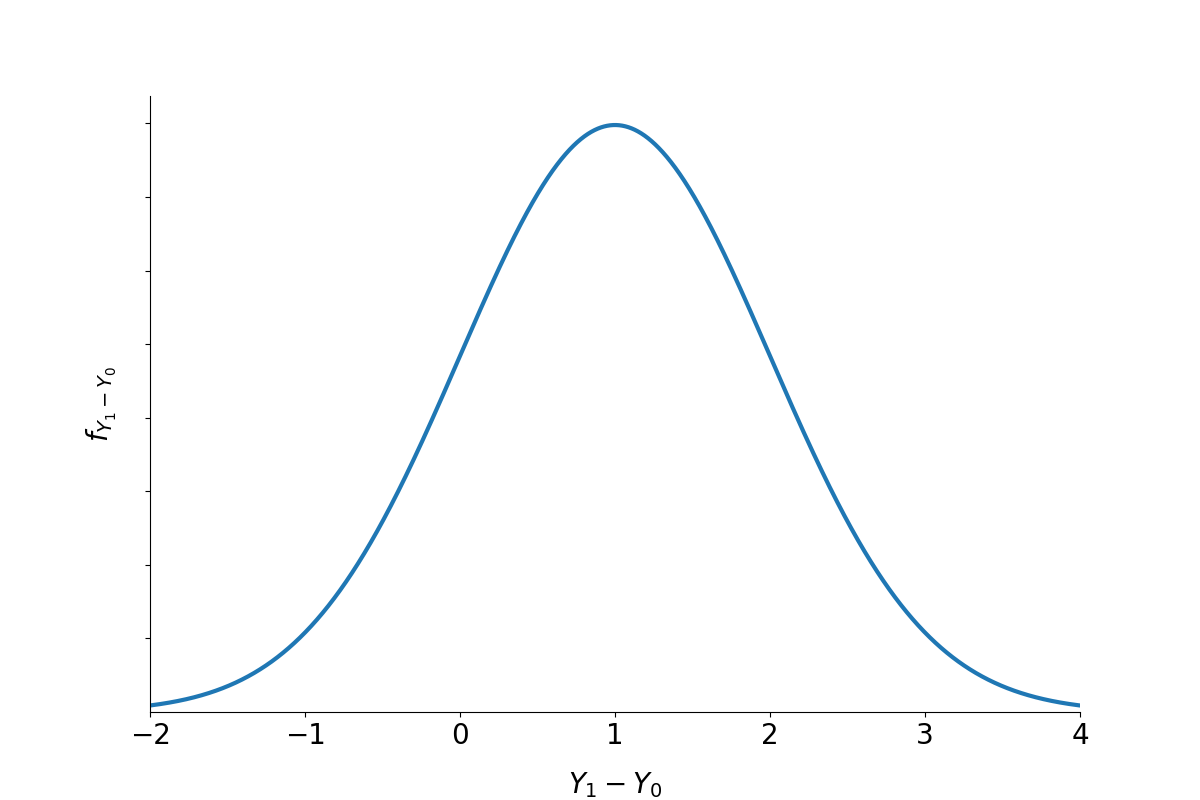
\includegraphics{fig-treatment-effects-benefits}}
\end{figure}
\end{frame}
%-------------------------------------------------------------------------------
%-------------------------------------------------------------------------------
\begin{frame}
	\begin{figure}\caption{Distribution of potential outcomes}
		\scalebox{0.35}{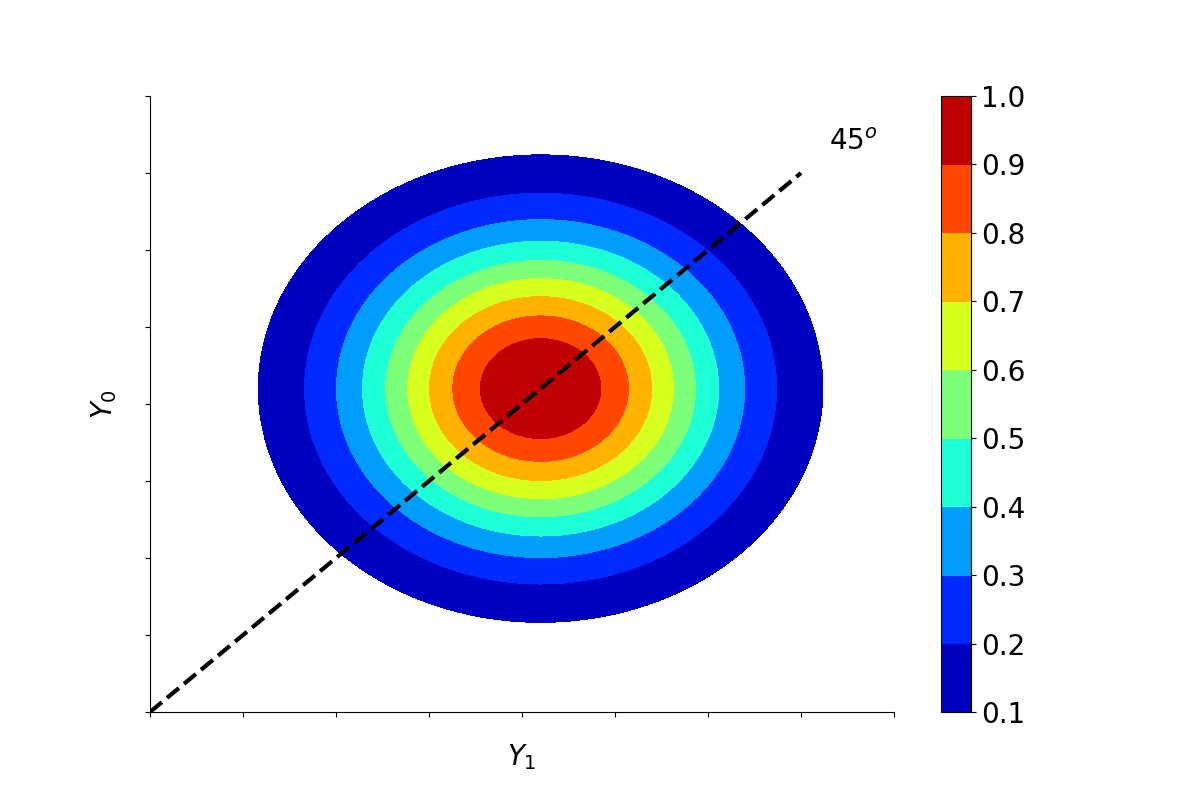
\includegraphics{fig-distribution-joint-potential}}
	\end{figure}
\end{frame}
%-------------------------------------------------------------------------------
%-------------------------------------------------------------------------------
\begin{frame}
	\begin{figure}\caption{Distribution of benefits and surplus}
		\scalebox{0.35}{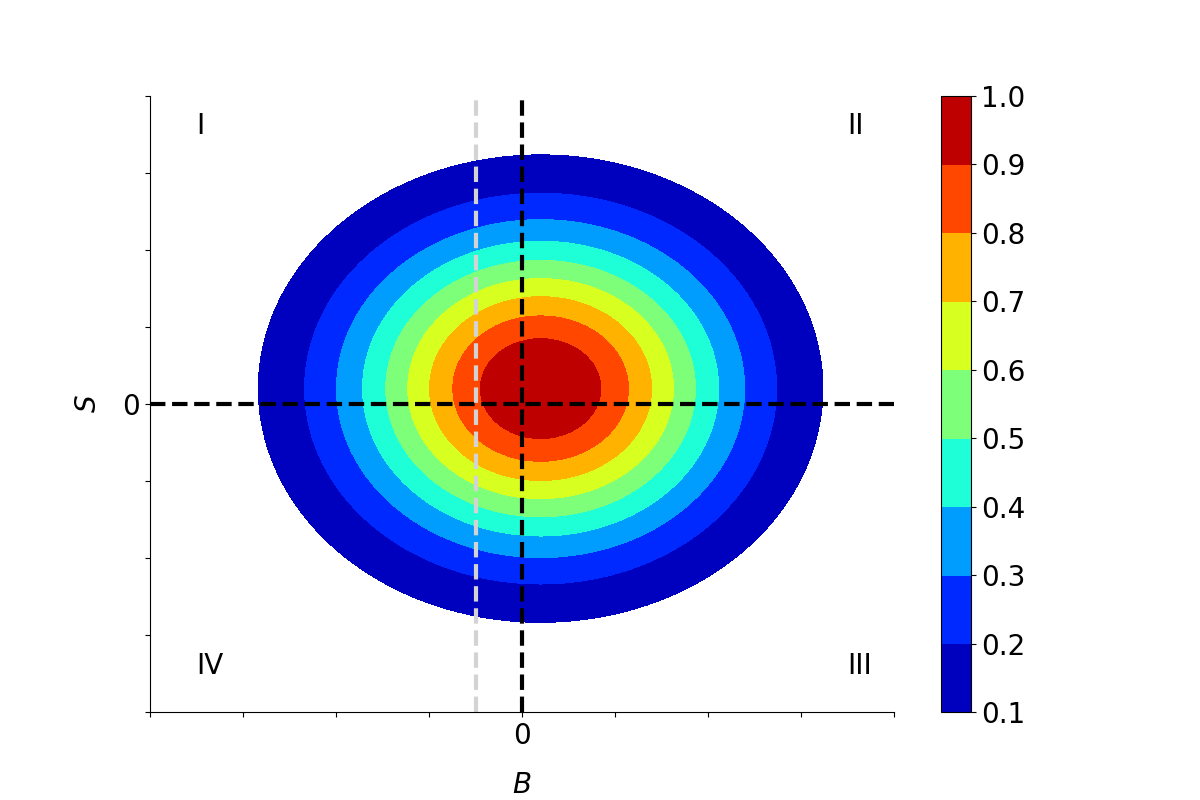
\includegraphics{fig-distribution-joint-surplus}}
	\end{figure}
\end{frame}
%-------------------------------------------------------------------------------
%-------------------------------------------------------------------------------
